\documentclass[a4paper, 11pt, oneside]{report} 
\usepackage[utf8]{inputenc}
\usepackage[dutch]{babel}
\usepackage{amsmath}
\usepackage{amsfonts}
\usepackage{amssymb}
\usepackage{graphicx}
\usepackage{caption}
\usepackage[table,xcdraw]{xcolor}
\usepackage[toc,page]{appendix}
\usepackage{hyperref}
\usepackage{titlesec}
\usepackage{listings}
\usepackage{float}
\usepackage{tikz}
\usetikzlibrary{trees}
\usepackage{tikz-qtree}
\usepackage{graphicx}
\usepackage{fancyref}
\usepackage{wrapfig}
\usepackage{url}
\usepackage{pdflscape}
\usepackage{fancyvrb}
\usepackage{fancyhdr}
\graphicspath{ {Afbeeldingen/} }
\usepackage{subfig}
\usepackage{tabularx}
\usepackage{apacite}
\usepackage{longtable}
\usepackage{titlecaps}
%\usepackage[T1]{fontenc}
\usepackage{titlesec, blindtext, color}
\definecolor{gray75}{gray}{0.75}
\newcommand{\hsp}{\hspace{20pt}}
\usepackage{pdfpages}


\newcolumntype{L}[1]{>{\raggedright\arraybackslash}p{#1}}

\titleformat{\chapter}[hang]{\huge\bfseries}{\thechapter\hsp\textcolor{gray75}{|}\hsp}{0pt}{\Large\bfseries}


\def\sectionautorefname{Paragraaf}
\def\chapterautorefname{Hoofdstuk}
\def\tableautorefname{Tabel}
\DeclareRobustCommand{\VAN}[3]{#2} % set up for citation

%% Sets page size and margins 
\usepackage[a4paper,top=3cm,bottom=3cm,left=3cm,right=3cm,marginparwidth=1.75cm]{geometry}

\author{M.W.J. Berentsen}
\font\myfont=cmr12 at 40pt
\title{\myfont Drone mesh netwerk simulatie}
\usepackage{titling}

\newcommand{\subtitle}[8]{%
	\posttitle{%
		\par\end{center}
	\begin{center}\large#1\end{center}
	\vskip0.5em
	\begin{center}\large#2\end{center}
	\begin{center}\large#3\end{center}
	\begin{center}\large#4\end{center}
    \begin{center}\large#5\end{center}
    \begin{center}\large#6\end{center}
    \begin{center}\large#7\end{center}
    \begin{center}\large#8\end{center}
	\vskip0.5em}%
}

\subtitle{Plan van aanpak}{HAN Arnhem}{561399}{MWJ.Berentsen@student.han.nl}{Versie 2}{Alten Nederland B.V.}{Docent: J. Visch, MSc}{Assessor: ir. C.G.R. van Uffelen}

\setlength{\parindent}{0pt}
\setlength{\parskip}{5pt plus 2pt minus 1pt}



\hypersetup{colorlinks=true, urlcolor=red,citecolor=black,linkcolor=blue}  % Colours hyperlinks in blue, but this can be distracting if there are many links.
\setcounter{tocdepth}{2}



\begin{document}
\begin{figure}
\begin{center}
\includegraphics[scale=0.1]{alten}\end{center}
\end{figure}
\maketitle

%\section*{Voorwoord}
%\addcontentsline{toc}{section}{\protect\numberline{}Voorwoord}
%\pagebreak

%Geschikt voor minimaal 50 nodes; Kan slecht of geen signaal nabootsen

\tableofcontents
\clearpage
%\section*{Begrippenlijst}

% Please add the following required packages to your document preamble:
% \usepackage[table,xcdraw]{xcolor}
% If you use beamer only pass "xcolor=table" option, i.e. \documentclass[xcolor=table]{beamer}
%\begin{table}[H]
%\centering

%\label{begrippen}
%\begin{tabular}{|l|l|}
%\hline
%\rowcolor[HTML]{C0C0C0}
%Term        & Omschrijving                                                         \\ \hline
%term        & Omschrijving                                                      	\\ \hline

%\end{tabular}
%\caption{Begrippenlijst}
%\end{table}

%\clearpage

%\section*{Samenvatting}
%\addcontentsline{toc}{section}{\protect\numberline{}Samenvatting}
%\pagebreak


\chapter{Inleiding}
\label{chapter:inleiding}
Het volgende verslag betreft het plan van aanpak voor de afstudeerstage van Maurice Berentsen (hierna: student).
Dit plan van aanpak is gebaseerd op het document \textit{"Toelichting op PvA 3.0"} \cite{HoePVA}

Het beschrijft de aanpak van de student waarin hij omschrijft wat hij gaat onderzoeken, 
hoe dit uitgevoerd wordt en wat de planning van het onderzoek is.

Drones zijn onbemande luchtvaartuigen die kunnen navigeren door de lucht en daarom toepasbaar om bepaalde taken uit te voeren voor de mens.
Alten wil gebruik maken van drones om een netwerk te kunnen creëren over een groot te gebied. 
Daarbij wil Alten dat dit netwerk zichzelf kan herstellen door drones te kunnen herpositioneren bij uitval of een slechte verbinding.
Het onderzoek die uitgevoerd gaat worden in dit luidt de volgende vraag:
\begin{quotation}
	\textit{Welke verdeel algoritme en extra intelligentie is nodig voor en netwerkmodule, aangesloten op een drone, om te zorgen voor een optimaal netwerk van drones in een gebied?}
\end{quotation}

Dit project heeft een tweedelig doel.
Het doel voor de student is het aantonen dat hij competent in zijn vak als embedded software developer en het behalen van zijn bachelor diploma Technische Informatica.
Het doel van de organisatie Alten Nederland BV. is het zetten van een eerste stap naar bouwen van een drone netwerk door een prototype van een netwerkmodule voor een drone op te leveren die het meshnetwerk opzet en wanneer nodig de drones kan herverdelen.

Omdat de uitvoerende student geen vergunning heeft om te vliegen met drones gebruikt hij een simulatie.
De simulatie heeft als doel om de verdeling van de drones te visualizeren, het gedrag te testen bij uitval of storing in het netwerk en simuleren van de drones zelf.

Er wordt voor de communicatie een fysiek prototype gemaakt.
Dit prototype zal bestaan uit microcontrollers die draadloos met elkaar communiceren via een onderling meshnetwerk. 
Dit prototype wordt niet alleen gemaakt voor het aantonen van de communicatie maar ook voor het extraheren van realistisch communicatie gedrag in de simulatie.

Een samenvatting van het plan is:

\begin{itemize}
	\item Onderzoek de keuze naar het gebruik van simulatiesoftware, hardware en software meshnetwerk en drone simulatie.
	\item Implementeer de drone in de simulatiesoftware; Bouw een prototype van het mesh netwerk en simuleer deze; Gebruik het netwerk om meerdere drones aan te sturen; Implementeer het gedrag van de drones binnen het netwerk voor verschillende usecases. %TODO link naar usecase
	\item Beantwoord de onderzoeksvraag en lever hiervoor een onderzoeksrapport op.
\end{itemize}

\section{Leeswijzer}

Dit document gaat eerst in op de \nameref{chapter:achtergrond} waar het bedrijf kort omschreven wordt en de aanleiding voor dit project.
Vervolgens gaat \autoref{chapter:doelstelling} in op het doel, de opdracht en het resultaat van het project.
Daarna is het project afgebakend in het hoofdstuk \nameref{chapter:projectgrenzen}.
Direct daarop zijn de \nameref{chapter:randvoorwaarden} naar zowel het bedrijf als de school vastgelegd.
Hierna is in \autoref{chapter:producten} per product, die de student wil opleveren, opgesteld wat de kwaliteitseisen zijn en hoe hij daar aan wil voldoen.
\autoref{chapter:ontwikkelmethode} verduidelijkt welke ontwikkelmethode de student gebruikt tijdens het project.
Een praktisch hoofdstuk wat betreft contactgegevens en onderlinge communicatie volgt hierop in \nameref{chapter:projectorganistatie}.
De \nameref{chapter:planning} is in het daarop volgende hoofdstuk uitgewerkt.
Tenslotte eindigt het plan van aanpak met een risicoanalyse in \autoref{chapter:risicos}.



\chapter{Achtergrond van het project}
\label{chapter:achtergrond}
Alten Nederland B.V. is een bedrijf met omstreeks 650 medewerkers in dienst. 
Overkoepelend is Alten Group die in totaal wereldwijd meer dan 25.000 engineers in dienst heeft.
De afdeling oost waar de stage plaats vindt telt ongeveer 50 medewerkers. 
Dit zijn grotendeels consulenten die meewerken aan de productontwikkeling van de partners van Alten op het gebied van technische software engineering.
Het overige deel is technisch management en human resource management.
\begin{figure}[H]
	\begin{center}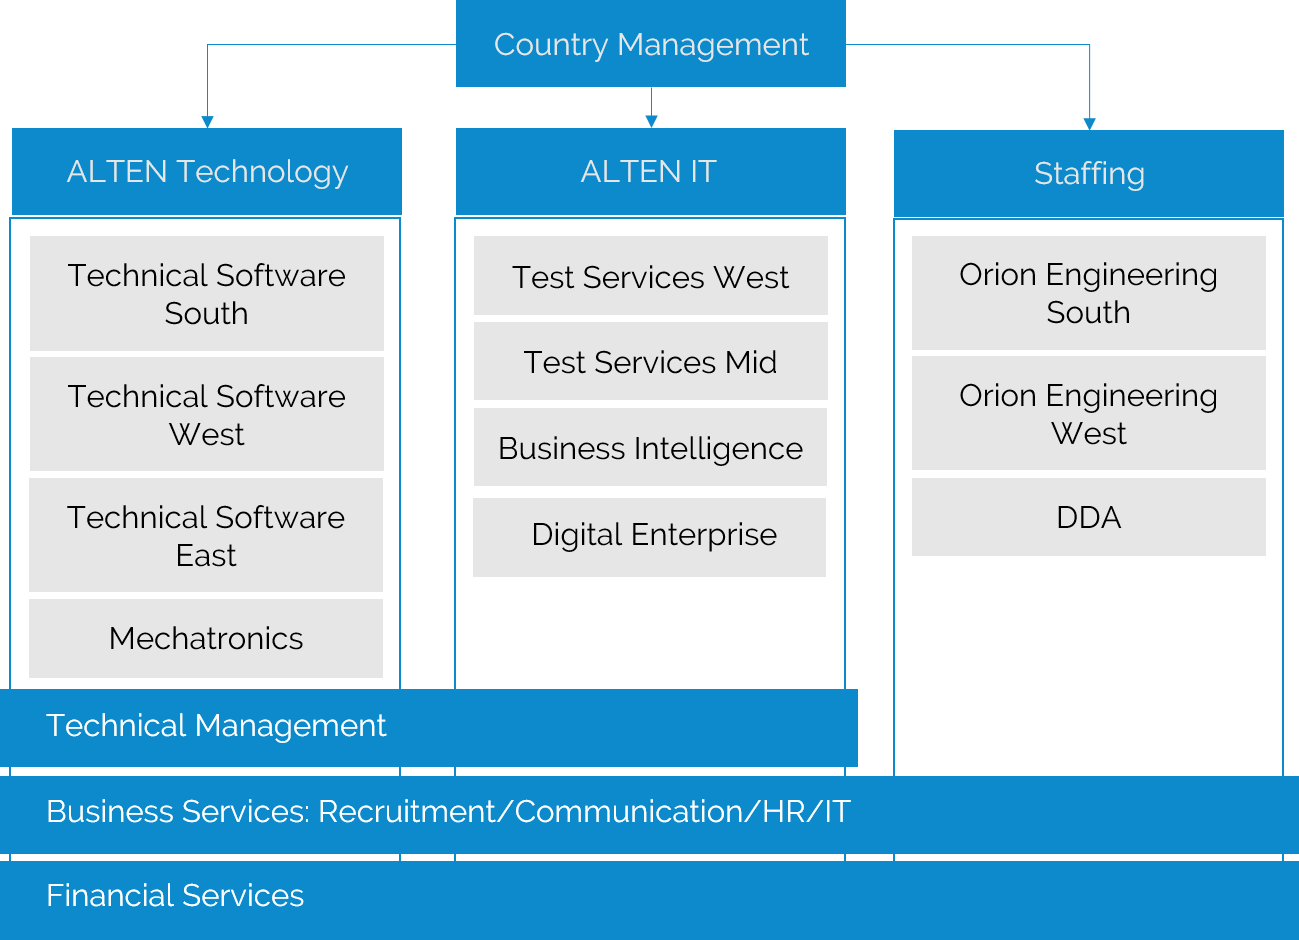
\includegraphics[scale=0.18]{organogram}\end{center}
	\caption{Organogram Alten IT. Afkomstig van \textit{intranet.alten.nl}, 5 februari 2019 }
	\label{fig:organogram}
\end{figure}

In figuur \ref{fig:organogram} is het organogram van Alten IT zichtbaar.
De student voert zijn onderzoek uit binnen het onderdeel Technical Software East.

De omzet van Alten haalt zij uit het delen van kennis door onder andere het detacheren van specialisten, uitvoeren van projecten of het geven van workshops.
Daarmee is kennis dus van groot belang voor Alten en is zij altijd bezig deze uit te breiden. 

Alten is in het bezit van drones en is bezig haar kennis hierin uitbreiden.
Deze kennis breidt zij uit door te investeren in onderzoeken naar dit onderwerp.

Het gebruik van drones neemt toe in Nederland.
Volgens het luchtvaartregister in de publicatie van \citeA{ILeT} zijn er op 03-10-2018 1806 drones geregistreerd. 
Daarmee is het aantal drones met een totaal aantal luchtvaart voertuigen van 4445 goed voor 40.6 procent.
Op 1 juni 2017 heeft \citeA{aantalDrones} van het mediabedrijf Dronewatch een zelfde berekening gedaan waarbij het aantal nog 755 drones was en goed voor 22 procent. Dit is dus een vervijfvoudiging in iets meer dan een jaar tijd.

Alten springt in op deze snel groei in toename van drones door zo snel mogelijk meer kennis op te doen naar dit onderwerp.
Het is daarom urgent voor Alten om te investeren in onderzoeken naar toepassingen van drones.

\chapter{Doelstelling, opdracht en op te leveren resultaten voor het bedrijf en school}
\label{chapter:doelstelling}
Het doel van Alten is om onderling verbonden drones kunnen verdelen om zo een netwerk op te kunnen bouwen over een gebied. 
Alten wil dat dit netwerk zichzelf kan onderhouden door te reageren op uitval of een slechte verbinding door de één of meerdere drones te herverdelen.

\section{Probleem}
Het probleem wat een dronenetwerk met zich meebrengt is dat er wellicht een drone kan uitvallen of dat een punt in het netwerk een slechte verbinding heeft. 
Op het moment dat dit gebeurd heeft het een negatieve impact op het hele netwerk, omdat er mogelijk andere drones afhankelijk zijn van dit communicatiepunt.
Een herverdeling van de drones is hiervoor een oplossing. Alleen wat is een efficiënte manier van herverdelen?
Het makkelijkste is om alle drones terug naar hun start punt laten vliegen maar dit zou betekenen dat het netwerk op dat moment niet beschikbaar is en het zou ook nog eens onnodig veel stroom verbruiken. 

\section{Doelstelling}
Het doel van dit project is dus om te onderzoeken wat een slimme manier is om de drones te herverdelen bij uitval. Alten wil deze intelligentie overlaten aan de netwerkmodule die toegevoegd moet worden aan de drone. Deze module bestaat nog niet en er moet dus een prototype gebouwd worden door de student. Hierbij hoeft de netwerkmodule alleen een nieuw coördinaat te geven aan de drone als een verplaatsing nodig is. Hoe de verplaatsing uitgevoerd wordt heeft geen betrekking op dit project. 

\section{Opdracht}
De opdracht van dit project is de ontwikkeling van meerdere producten die bijdragen aan het behalen van het doel. 
De afstudeerder moet een algoritme maken die bepaald hoe de drones zich moeten verdelen in een gebied en hoe ze moeten reageren bij uitval of slechte verbinding.
Een gebruiker moet kunnen aangeven over wat voor een gebied de drones zich moeten verdelen.
Dit gebied bestaat uit een vrije vorm zoals een cirkel, hoefijzer, vierkant of donut.

Er moet een prototype gemaakt worden van een netwerkmodule die het onderlinge meshnetwerk verzorgt en zichzelf kan herstellen bij uitval maar wel een andere communicatie route mogelijk is. 
Wanneer dit niet het geval is moet de module de drone herpositioneren.

Tenslotte moet de student een simulatie opzetten waarin al het bovenstaande gedrag in terug komt. 
Deze simulatie is nuttig voor het testen van het verdelingsalgoritme en het visualiseren van het netwerk.
Alten wil graag dat de simulatie uitgevoerd wordt in Robot Operating System (ROS). 
Dit wil Alten omdat zij nog geen ervaring heeft in ROS in combinatie met drones en mesh netwerken en door het begeleiden hier ervaring in opdoet.
Het ervaring opdoen in ROS is geen doel van dit project en de student hoeft zich niet op te concentreren.
De simulatie zal bestaan uit een stuk waar de input van de gebruiker ingevoerd kan worden, en een stuk waar een instelbaar aantal drones zich zullen verdelen over het opgegeven gebied.

De simulatie moet realistisch en valide zijn.
Dit houdt voor dit project in dat de drones met elkaar communiceren via een gesimuleerd mesh netwerk. 
De drones moeten in de simulatie kunnen uitvallen en de onderlinge afstand heeft effect op de signaalsterkte.
De simulatie moet aan de hand van een script herhaalbaar zijn met een zelfde resultaat.
 

Alten heeft geen eigen software producten op de markt.
Het bedrijf heeft daarom op dit moment ook geen interesse om dit product op de markt te zetten.

\section{Op te leveren resultaten voor het bedrijf en school}

Aan het einde van het project levert de student de volgende producten op aan het bedrijf:

\begin{itemize}
\item Simulatiesoftware met meerdere drones en netwerksimulatie
\item Prototype meshnetwerk module.
\item Broncode van de bovenstaande producten. 
\item SRS (Software Requirement Specification)
\item SDD (Software Design Document)
\item Onderzoeksverslag
\end{itemize}

Aan het einde van het project levert de student het bovenstaande plus een projectverslag op aan de Hogeschool van Arnhem en Nijmegen.

\chapter{Projectgrenzen}
\label{chapter:projectgrenzen}
Om duidelijkheid te scheppen in dit project zullen hier de grenzen van het project besproken worden.
Dit is om voor beide partijen duidelijkheid te creëren welke zaken er niet uitgevoerd gaan worden. 

Deze grenzen zijn onderverdeelt in:

\begin{itemize}
	\item Organisatorische grenzen.
	\item Inhoudelijke grenzen.
\end{itemize}

\section{Organisatorische grenzen}
Hier staan alle grenzen die organisatorische invloed hebben. 

\begin{itemize}
	\item Het project start op 1 februari 2019.
	\item Het project stopt op 28 juni 2019.
	\item De student werkt 5 dagen per week aan het project wat een totaal van 40 uur per week geeft.
	\item Het project wordt door één student uitgevoerd.
	\item De locatie waar de student werkt is vrij waarbij de werkplek van Alten voorkeur heeft.
	\item Het schoolritme dicteert gedurende het project, ofwel tijdens de schoolvakanties is de student vrij.
\end{itemize}

\section{Inhoudelijke grenzen}
Hier staan alle grenzen die inhoudelijk over het project gaan. In hoofdstuk \ref{chapter:doelstelling} is te vinden welke producten worden opgeleverd. Daarnaast zullen ook de volgende punten onder de inhoudelijke project grenzen vallen.

\begin{itemize}
	\item In het project wordt niet met fysieke drones gevlogen.
	\item Het verdelingsalgoritme wordt alleen in een simulatie aangetoond
	\item De simulatie dient alleen het doel van het beantwoorden van de onderzoeksvraag.
	\item De simulatie zal niet meer dan 100 drones gelijktijdig simuleren door de limieten van de simulatiesoftware.
	\item De simulatie zal alleen situaties nabootsen die echt kunnen gebeuren.
	\item De simulatie bootst alleen een grote vlakke ruimte na waar de drones in gaan vliegen en parkeren.
	\item Als middleware voor de simulatie moet ROS gebruikt worden om de kennis van Alten uit te breiden.
	\item De simulatie zal alleen drones en een vlak grond gebied simuleren.
	\item Er is geen beschikbaar budget afgesproken met de Alten. De student maakt geen eigen kosten ten behoeve van de uitvoer van het	project. 
	\item Versiebeheer voor code maar ook documenten vindt plaats op de repository van het stage aanbiedende bedrijf.
	\item Na de einddatum en wanneer alle resultaten geleverd zijn zal er geen nazorg meer geleverd
	worden door de afstudeerder aan het project binnen het huidige dienstverband.
	\item Documentatie wordt geschreven in latex om het voor de student gemakkelijk te maken algoritmes te documenteren.
	\item Code wordt geschreven in C$++$ omdat dit hoort bij de specialisatie van de student als embedded software developer.
	\item Er wordt één soort prototype netwerkmodule gemaakt.
\end{itemize}

\chapter{Randvoorwaarden}
\label{chapter:randvoorwaarden}
Bij randvoorwaarden geeft de student aan welke zaken er door de opdrachtgever geregeld moeten worden voordat hij aan het project kan beginnen. De student heeft randvoorwaarden opgedeeld in organisatorische en inhoudelijke randvoorwaarden. 

\section{Organisatorische randvoorwaarden}
\begin{itemize}
	\item Beschikbaarheid van de HAN procesbegeleider: Alle werkdagen per mail waarop binnen 72 uur geantwoord wordt, bereidt om naar Alten te reizen op de feedbackmomenten.
	\item Alten stelt vijf dagen per week een werkplek met een internetverbinding beschikbaar.
	\item Contactgegevens van alle betrokken partijen zijn bekend bij elkaar.
	\item Begeleiders zijn in het bezit van een GitHub account en maken deze ook bekend aan de student.
	\item De student krijgt de ruimte om aan zijn verslagen voor school te werken binnen de 40 uur durende werkweek.
	
\end{itemize}
\section{Inhoudelijke randvoorwaarden}
\begin{itemize}
	\item Beschikbaarheid van de bedrijfsbegeleider: Alle werkdagen per mail waarop binnen 48 uur geantwoord wordt, eenmaal per week overleg/reflectie met de student.
	\item Alten verzorgt een laptop krachtig genoeg voor simulaties voor de student.
	\item De HAN procesbegeleider beoordeelt documentatie op ISAS binnen het door het systeem opgeven termijn.
	\item Afstudeerder moet de kans krijgen om tijdens het project de competenties gesteld vanuit de
	opleiding te kunnen behalen, en aan te kunnen tonen.
\end{itemize}

\chapter{Op te leveren producten en kwaliteitseisen}
\label{chapter:producten}
In dit hoofdstuk worden de op te leveren producten, kwaliteitseisen en de uit te voeren activiteiten besproken.
Het gaat hier om zowel de producten die aan de opdrachtgever worden opgeleverd, als om de producten die voor school worden opgeleverd.
Hierbij worden de resultaten, zoals beschreven in \autoref{chapter:doelstelling}, nader uitgewerkt.
Voor alle producten worden kwaliteitseisen opgesteld, waaraan de producten moeten voldoen.
Daarnaast worden ook alle overige activiteiten aangehaald in dit hoofdstuk om te komen tot het product.

Alle documentatie die wordt geschreven voldoet aan de kwaliteitseisen van de ICA controlekaart.

% Please add the following required packages to your document preamble:
% \usepackage[table,xcdraw]{xcolor}
% If you use beamer only pass "xcolor=table" option, i.e. \documentclass[xcolor=table]{beamer}
\begin{longtable}[c]{|l|l|l|l|l|}
	\hline
	\rowcolor[HTML]{C0C0C0} 
	\centering
	Product          & Productkwaliteit eisen	& \begin{tabular}[c]{@{}l@{}}Benodigde activiteiten \\ om te komen tot \\ het product\end{tabular}                                                                             & Proceskwaliteit                                                                                                                                        \\ \hline	\endhead
	Broncode                                                                                                   & \begin{tabular}[c]{@{}l@{}}Komt overeen met SRS en\\ SDD; Alle publieke functies \\ zijn voorzien van Engels\\ commentaar; Kritische\\ functies  hebben unit tests; \\ Voldoet aan de code\\ standaard van \autoref{app:code};\\ De \nameref{app:DoD}\\ is voldaan \end{tabular}           & \begin{tabular}[c]{@{}l@{}}Schrijven code;\\ Opstellen code\\ standaard; Unit\\ testen schrijven;\\ Commentaar in\\ code schrijven.\end{tabular}                             & \begin{tabular}[c]{@{}l@{}}Wekelijks code\\ reviews; Tussentijdse\\ beoordeling door\\  begeleiders; Het \\ gebruik van code\\ analysetool \href{http://cppcheck.sourceforge.net/}{Cppcheck}.\\ Invullen van de\\ \nameref{app:DoD} \end{tabular}                                      \\ \hline
	\begin{tabular}[c]{@{}l@{}}Presentatie /\\ verdediging\end{tabular}                                    & \begin{tabular}[c]{@{}l@{}}Ondersteunt het \\ projectverslag in het\\ aantonen van de vijf \\ beoordelingscriteria;\\ \cite{HANbc} \\ Geeft een indruk van het\\ opgeleverde product;\\ Duurt in totaal niet \\langer dan 30 minuten.\end{tabular} & \begin{tabular}[c]{@{}l@{}}Presentatie maken;\\ Demonstratie van\\ het product maken.\end{tabular}                                                                                   & \begin{tabular}[c]{@{}l@{}}Oefenen met\\ bedrijfsbegeleiders\\ /collega’s.\end{tabular}                                                                
	\\ \hline
	\begin{tabular}[c]{@{}l@{}}Plan van\\ aanpak \end{tabular}                                                                                             & \begin{tabular}[c]{@{}l@{}}Omschrijft wat het plan\\ van de  student is; Voldoet \\aan het  feedbackformulier \\ projectplan van het\\\citeauthor{HANfeed}\\\citeyear{HANfeed}  .\end{tabular}                                                                                          & \begin{tabular}[c]{@{}l@{}}Verdiepen in het\\ stage aanbiedende\\ bedrijf;\\ Verduidelijken\\ stageopdracht;\\ Het plan schrijven.\end{tabular}                              & \begin{tabular}[c]{@{}l@{}}Feedback/goedkeuring\\ van bedrijfsbegeleider;\\ Feedback van\\ procesbegeleider en \\ assessor;\end{tabular}
	\\ \hline
	Projectverslag                                                                                             & \begin{tabular}[c]{@{}l@{}}Toont de vijf\\ beoordelingscriteria met\\ bijhorende prestatiecriterium\\ \cite{HANbc} \\ voldoende aan; Onderbouwt\\ de keuzes van handelen.\end{tabular}                                                             & \begin{tabular}[c]{@{}l@{}}Keuzes tijdens het\\ project documenteren;\\ Feedback gesprekken\\ houden; Het schrijven\\ van het verslag\end{tabular}                           & \begin{tabular}[c]{@{}l@{}}Tussentijdse \\ feedbackrondes; \\ Feedback van de \\ procesbegeleider; \\ Wekelijkse \\ feedbacksessie Alten.\end{tabular}
	\\ \hline
	\begin{tabular}[c]{@{}l@{}}Prototype\\ mesh\\ netwerk\end{tabular}                                           & \begin{tabular}[c]{@{}l@{}}Geschikt om gedrag te\\ extraheren voor de simulatie; \\ Voldoet aan de opgestelde\\ requirements van het\\ dronenetwerk.\end{tabular}                                                        & \begin{tabular}[c]{@{}l@{}}Keuze maken in\\ hardware gebruik;\\ Software voor\\ onderzoek schrijven;\\ Onderzoek naar\\ gedrag van het \\ netwerk.\end{tabular}              & \begin{tabular}[c]{@{}l@{}}Code reviews; feedback\\ op onderzoek van\\ begeleiding.\end{tabular}                                                       
	\\ \hline
	\begin{tabular}[c]{@{}l@{}}
		Onderzoeks-\\ verslag                    
	\end{tabular}                                                                      & \begin{tabular}[c]{@{}l@{}}Bevat een relevante \\ onderzoeksvraag; \\ Geeft antwoord op de\\ onderzoeksvraag;  Is\\ gebaseerd op de \\ ICA-onderzoek kaart.\\ \cite{MethodenKaart}\\\end{tabular} & \begin{tabular}[c]{@{}l@{}}Zowel literatuur-\\ als labonderzoek\\ uitvoeren;\\ Software bouwen\\ voor het bewijzen\\ van het antwoord.\end{tabular}                         & \begin{tabular}[c]{@{}l@{}}Wekelijks reflecteren\\ met de stagebegeleider\\ op het proces van het \\ onderzoek.\end{tabular}   
	\\ \hline
	\begin{tabular}[c]{@{}l@{}}Simulatie \\software\\ met meerdere \\ drones en \\ netwerk\\ simulatie\end{tabular} & \begin{tabular}[c]{@{}l@{}}Realistisch en valide;\\ Geschikt om de \\ onderzoeksvraag te \\ beantwoorden; Is voorzien\\ van  documentatie.\end{tabular}                                                      & \begin{tabular}[c]{@{}l@{}}Schrijven van\\ code; Onderzoek\\ doen wanneer de\\simulatie realistisch\\en valide is; Gedrag\\ van het netwerk \\ overzetten tot \\ gesimuleerd gedrag;\\ Een drone simuleren.\end{tabular}                   & \begin{tabular}[c]{@{}l@{}}Code reviews; \\ Terugkoppeling van\\het product naar\\Alten.\end{tabular}                                        
	\\ \hline
	\begin{tabular}[c]{@{}l@{}}Software \\Design\\ Document\end{tabular}                                         & \begin{tabular}[c]{@{}l@{}}Komt overeen met\\ code; Toont alle\\ relevante ontwerpen; \\ Ontwerpkeuzes staan\\  vastgelegd.\end{tabular}                                                                        & \begin{tabular}[c]{@{}l@{}}Usecases vertalen tot\\ activity diagrammen;  \\ Domein model \\ omzetten tot class\\ diagrammen; \\ component diagram\\  opstellen.\end{tabular} & \begin{tabular}[c]{@{}l@{}}Ontwerpkeuzes \\ bespreken met\\ begeleiding; \\ Ontwerp baseren\\ op ontwerppatronen.\end{tabular} 
	\\ \hline
	\begin{tabular}[c]{@{}l@{}}Software \\ Requirement \\ Specification\end{tabular}                           & \begin{tabular}[c]{@{}l@{}}De requirements\\ komen overeen met\\ de wensen van de \\ opdrachtgever; Bevat \\genoeg informatie\\ voor het opstellen\\ van een SDD.\end{tabular}                                   & \begin{tabular}[c]{@{}l@{}}Eisen van het \\ product vaststellen;\\ usecases opstellen;\\ furps++ opstellen.\end{tabular}                                                     & \begin{tabular}[c]{@{}l@{}}Producteisen en\\ usescases terugkoppelen \\naar de opdrachtgever.\end{tabular}           
	\\ \hline
	\caption{Op te leveren producten met gestelde eisen m.b.t. activiteit en kwaliteit}
\end{longtable}




\chapter{Ontwikkelmethoden}
\label{chapter:ontwikkelmethode}
De genoemde op te leveren producten in het voorgaande hoofdstuk worden gerealiseerd door middel van de ontwikkelmethoden RUP in combinatie met scrum.

Deze ontwikkelmethode geeft de student de mogelijkheid om voldoende onderzoek te doen naar de problemen die deze opdracht met zich mee brengt. 
Binnen RUP wordt er ook aan het einde van iedere iteratie een retrospectieve en een review gehouden. Tijdens deze retrospectieven en reviews wordt de voortgang van het proces en het product besproken. Hierdoor krijgt de student niet alleen een duidelijk beeld van de staat van het te ontwikkelen product, maar ook van de afgeronde competenties. Hierdoor kan de student vervolgens bijsturen wanneer nodig om de benodigde competenties te halen.

\section{Rational Unified Process} 

RUP (Rational Unified Process) is een iteratieve ontwikkelmethode. Dit houdt in dat het project
wordt gerealiseerd in verschillende, elkaar opvolgende iteraties en dat ervaringen uit voorgaande iteraties in volgende iteraties worden meegenomen.\cite{RUP}

\subsection{De vier fases van RUP}
\label{sec:fasesRUP}
RUP beschrijft vier fasen waarin de nadruk ligt op verschillende disciplines van RUP \cite{RUPwim}.
Hieronder de vier fasen, hoelang ze duren en een korte beschrijving.

\subsubsection{Inceptionfase}
\label{sec:inceptionfase}
De inceptiefase loopt tot en met 15 maart en duurt 5 weken.

In deze periode gaat de student de scope, doelen, projectgrenzen, risico's en tegenmaatregelen vastleggen.
Deze worden vast gelegd in het plan van aanpak.
Aan het einde van de inceptie fase is er een analyse gemaakt en zijn de eisen bekend.
Ook zijn er ideeën bedacht over hoe het systeem geïmplementeerd moet worden.

\subsubsection{Elaborationfase}
\label{sec:elaborationfase}
Deze fase eindigt op 17 mei  en duurt 8 weken.

In deze fase worden de bedachten ideeën uit de inceptiefase uitgewerkt.
Er worden prototypes gemaakt en onderzoeken gedaan om te kijken of bepaalde dingen mogelijk zijn.
Aan het einde van de elaboratie fase is het bekend hoe het systeem wordt gerealiseerd en bestaat er een stabiele architectuur.
Met stabiele architectuur wordt bedoelt dat er een versie bestaat van het systeem, waarbij er door op ontwikkeld kan worden.
De elaboration fase is opgedeeld in vier iteraties van twee weken.

\subsubsection{Constructionfase}
\label{sec:constructionfase}
Deze fase duurt 4 weken en is klaar op 14 juni.

In deze fase wordt het systeem gerealiseerd. De constructie fase bestaat uit iteraties van een week.
Volgens het onderwijs moet op vrijdag 14 juni alles op ISAS ingeleverd zijn, tot die tijd wordt alles afgerond.
Aan het einde van deze fase is het proof of concept aanwezig en voldoet deze aan de gestelde kwaliteitseisen, zoals gesteld in \autoref{chapter:producten}.
Tevens wordt er een onderzoeksrapport opgeleverd waarin de eerder genoemde gestelde vragen beantwoord worden.

\subsubsection{Transistionfase}
Deze fase loopt van 17 juni tot 27 juni.

In de transitiefase wordt de presentatie en demo voorbereid. 
In deze fase wordt het systeem gepresenteerd aan de opdrachtgever en school.

\subsection{Risicovermindering}
\citeauthor{IBMrup}\citeyear{IBMrup} beschijft dat RUP een algemene benadering heeft wat betreft risico's. De risico's worden geïdentificeerd en er worden uitwijkstrategieën opgesteld. De risico's worden gebruikt bij het prioriteren van de use cases en de risico's worden meegenomen als doelen voor het beoordelen van een iteratie. Tijdens de inceptionfase worden de grootste risico's beschreven. In de elboratiefase worden risico's afgedekt door middel van proof of concepts.

\subsection{Templates}
Templates helpen met het stroomlijnen van het proces tijdens het project. RUP heeft een ruim aanbod van templates. Niet iedere template is relevant voor dit project. In dit hoofdstuk worden de templates behandeld die de student wil gebruiken in dit project.

De volgende templates worden gebruikt tijdens het project.

\subsubsection{Iteratieplan template}

De iteratie template is handig te gebruiken, omdat hierin  wordt vastgelegd wat de doelen van de iteratie zijn. De iteratie template is uit RUP gehaald.

\autoref{app:iteratieplan} \nameref{app:iteratieplan}

\subsubsection{Iteration Assessment template}

Aan het einde van een iteratie geëvalueerd hoe de iteratie is gegaan en wat er verbeterd kan worden. Om dit proces te structureren beschrijft RUP een 'Iteration Assessment template' hier worden actiepunten opgesteld en opgeschreven wat er gehaald is en wat niet.

\autoref{app:assesement} \nameref{app:assesement}
\subsubsection{Use Case template }

Voor use cases gebruiken wordt er een zelfgemaakt template gebruikt. Dit template is gebaseerd op kennis uit het OSM semester en beschrijft voor een use case verschillende zaken zoals de actors, stakeholders en de flow.

\autoref{app:usecasetemplate} \nameref{app:usecasetemplate}

\section{De aspecten van scrum}
Net als RUP is scrum een agile framework die op een iteratieve manier te werk gaat.
Zo hebben beide ontwikkelmethoden iteraties.
Scrum is meer gericht op dagelijkse taken in tegenstelling to RUP waarbij dit niet het geval is.
Scrum vereist dat het op te leveren product ten alle tijden potentially shippable is \cite{james}. 
Dit betekent dat bij scrum het product continu goed geïntegreerd en getest moet zijn bij iedere iteratie. 

Omdat dit project door één student wordt uitgevoerd zijn niet alle best practices van scrum van toegevoegde waarde en zijn daarom weggelaten.
In de onderstaande \autoref{table:scrum} worden de aspecten van scrum aangekaart welke gebruikt worden in dit project.

\begin{table}[H]
	\centering
	\begin{tabular}{|l|l|l|}
		\hline
		\rowcolor[HTML]{C0C0C0} 
		Element            & Wat houdt het in                                                                                                                                       & Waarom?                                                                                                                         \\ \hline
		Sprint Review      & \begin{tabular}[c]{@{}l@{}}Presentatie van product\\ en voortgang aan de \\ opdrachtgever \& andere\\ belanghebbenden\end{tabular}                     & \begin{tabular}[c]{@{}l@{}}Om feedback te krijgen\\ van de opdrachtgever en\\ de prioriteiten te controleren\end{tabular}       
		\\ \hline
		Retrospective      & \begin{tabular}[c]{@{}l@{}}Bespreking van proces. \\ Wat ging goed/fout en wat gaat\\  de student volgende keer beter doen?\end{tabular}               & \begin{tabular}[c]{@{}l@{}}Om het proces van het\\ project te verbeteren.\\ Proces heeft invloed\\ op het product.\end{tabular} 
		\\ \hline
		Product backlog    & Lijst met gewenste functionaliteit.                                                                                                                    &                                                                                                                    \\ \hline
		Sprint backlog     & \begin{tabular}[c]{@{}l@{}}Scrum board met taken\\ bestaande uit de kolommen: \\ Todo - busy - for review - done\end{tabular}                          & \begin{tabular}[c]{@{}l@{}}Overzicht houden in\\ de voortgang van taken\end{tabular}                           
		\\ \hline
		Burn down chart     & \begin{tabular}[c]{@{}l@{}}Grafiek die weergeeft wat er nog\\ gedaan moet worden.\end{tabular}                          & \begin{tabular}[c]{@{}l@{}}Toont in een oogopslag hoe\\ een sprint er voor staat en\\ de planning gehaald wordt.\end{tabular}                           
		\\ \hline
		Sprint planning     & \begin{tabular}[c]{@{}l@{}}Een detail planning\\ voor de sprint.\end{tabular}& \begin{tabular}[c]{@{}l@{}}Geeft overzicht en focus over\\ de te behalen doelen van de\\ sprint. \end{tabular}                           
		\\ \hline
		Definition of Done   & \begin{tabular}[c]{@{}l@{}}Een checklist om te controleren\\ of een programmeer taak klaar is.\end{tabular}& \begin{tabular}[c]{@{}l@{}}Voorkomt dat taken\\ vergeten worden. \end{tabular}                           
		\\ \hline
	\end{tabular}
\caption{Overzicht elementen meegenomen uit scrum}
	\label{table:scrum}
\end{table}

\chapter{Projectorganisatie en communicatie}
\label{chapter:projectorganistatie}

Het volgende hoofdstuk gaat in op praktische informatie als contactinformatie en vakantiedagen. Daarnaast worden overige afspraken vastgelegd waar in staat hoe er in bepaalde situaties gehandeld moet worden.

\section{Begeleiders}
\label{sec:begeleiders}
Gedurende het project zijn er twee docenten van de HAN betrokken en twee medewerkers van Alten Nederland B.V..

\begin{table}[H]
	\centering
	\begin{tabular}{|l|l|l|l|}
		\hline
		\rowcolor[HTML]{C0C0C0} 
		Organistatie                                                                   & Naam                                                        & Rol                & Contact                  \\ \hline
		\begin{tabular}[c]{@{}l@{}}Hogeschool\\ van Arnhem \\ en Nijmegen\end{tabular} & \begin{tabular}[c]{@{}l@{}}Chris van\\ Uffelen\end{tabular} & Assessor           & 		\href{mailto:Chris.vanUffelen@han.nl}{Chris.vanUffelen@han.nl}   \\ \hline
		\begin{tabular}[c]{@{}l@{}}Hogeschool\\ van Arnhem \\ en Nijmegen\end{tabular} & Jorg Visch                                                  & Processbegeleider  & 
		\href{mailto:Jorg.Visch@han.nl}{Jorg.Visch@han.nl}   \\ \hline
		HAN / Alten                                                                    & Maurice Berentsen                                           & Afstudeerder       & \href{mailto:mauriceberentsen@live.nl}{mauriceberentsen@live.nl}   \\ \hline
		\begin{tabular}[c]{@{}l@{}}Alten \\ Nederland B.V.\end{tabular}                & Hugo Logmans                                                & Technisch Manager  &  \href{mailto:hugo.logmans@alten.nl}{hugo.logmans@alten.nl}   \\ \hline
		\begin{tabular}[c]{@{}l@{}}Alten \\ Nederland B.V.\end{tabular}                & Hugo Heutinck                                               & Bedrijfsbegeleider & \href{mailto:hugo.heutinck@alten.nl}{hugo.heutinck@alten.nl}   \\ \hline
	\end{tabular}
\caption{Contactinformatie alle betrokkenen bij dit project}
\label{table:begeleiders}
\end{table}

\section{Beschikbaarheid}
In \autoref{table:beschikbaarheid} staat beschreven wanneer de student aanwezig dient te zijn.

\begin{table}[H]
	\centering
	\begin{tabular}{|l|l|l|}
		\hline
		\rowcolor[HTML]{C0C0C0} 
		Dag                 & Aanwezig     & Locatie                                        \\ \hline
		Maandag t/m Vrijdag & 9:00 - 17:00 & Linie 544, 7325 DZ Apeldoorn 					\\ \hline
		Zaterdag en Zondag  & Vrij         & N.V.T.                                         \\ \hline
	\end{tabular}
\caption{Beschikbaarheid student gedurende het project}
\label{table:beschikbaarheid}
\end{table}

\section{Vrije dagen}

\autoref{table:vrijedagen} beschrijft welke dagen de student vrij heeft vanwege verplichte vrije dagen of schoolvakanties.

\begin{table}[H]
	\centering
	\begin{tabular}{|l|l|}
		\hline
		\rowcolor[HTML]{C0C0C0} 
		Toelichting           & Datum                           \\ \hline
		Voorjaarsvakantie     & 04-03-2019 - 10-03-2019 		\\ \hline
		Goede Vrijdag         & 19-04-2019                      \\ \hline
		2e Paasdag            & 22-04-2019                      \\ \hline
		Meivakantie           & 29-04-2019 - 05-05-2019         \\ \hline
		Hemelvaartsdag        & 30-05-2019                      \\ \hline
		Dag na Hemelvaartsdag & 31-05-2019                      \\ \hline
		2e Pinksterdag        & 10-06-2019                      \\ \hline
	\end{tabular}
\caption{Schoolvakanties en verplichte vrije dagen}
\label{table:vrijedagen}
\end{table}

Deze afwezigheid door verplichte vrije dagen telt bij elkaar een volledige werkweek op die de student afwezig is.
Omdat deze dagen goed zijn verdeelt over de RUP fases hebben ze weinig impact en wordt er niet speciaal op gepland.

\section{Overige afspraken}
Om de student zo goed als mogelijk te kunnen begeleiden zijn de overige afspraken opgesteld in \autoref{table:overigeafspraken}.
\begin{table}[H]
	\centering
	\begin{tabular}{|l|l|}
		\hline
		\rowcolor[HTML]{C0C0C0} 
		Onderwerp                                                               & Afspraak                                                                                                                                                                                                                                                                                       \\ \hline
		Ziekteverzuim                                                           & \begin{tabular}[c]{@{}l@{}}Bij ziekte maakt de student dit voor 09:00 telefonisch bekend aan zijn \\manager. Bij langdurige ziekte maakt de student
		 dit ook bekend aan\\ alle begeleiders
	 	\end{tabular}                                                                                                                                                                     \\ \hline
		\begin{tabular}[c]{@{}l@{}}Langdurige afwezig\\  of ziekte van \\ begeleiding\end{tabular} & \begin{tabular}[c]{@{}l@{}}Bij langdurige afwezigheid maakt de begeleider van de school of het bedrijf\\ dit bekend aan de student per mail. Bij afwezigheid langer dan twee weken \\moet de organistatie een tijdelijke vervanger aanbieden.\end{tabular}                                    \\ \hline
		Iteratie start                                                          & Iedere iteratie start op maandagochtend om 09:00                                                                                                                                                                                                                                               \\ \hline
		Werkplek                                                                & \begin{tabular}[c]{@{}l@{}}Er wordt van de student verwacht dat hij werkt op zijn werkplek bij Alten\\ in Apeldoorn. Op het moment dat dit afwijkt om bijvoorbeeld thuis te\\ werken laat hij dit minimaal een werkdag van te voren weten aan de stage\\ aanbiedende organisatie\end{tabular} \\ \hline
		\begin{tabular}[c]{@{}l@{}}Workshops en \\ terugkomdag\end{tabular}     & \begin{tabular}[c]{@{}l@{}}De student is vrij om de terugkomdag en workshops verzorgd door de HAN\\ bij te wonen. Wel laat hij dit tijdig weten aan de stage aanbiedende\\ organisatie. \end{tabular}                                                                                                                                                                  \\ \hline
		\begin{tabular}[c]{@{}l@{}} Code \end{tabular}     & \begin{tabular}[c]{@{}l@{}}De student gebruikt in het project C++ als programmeertaal.\\ Dit omdat dit past bij zijn specialisatie als embedded software developer \end{tabular}                                                                                                                                                                  \\ \hline
		\begin{tabular}[c]{@{}l@{}} IDE \end{tabular}     & \begin{tabular}[c]{@{}l@{}}De student is vrij in zijn keuze van IDE. \end{tabular}                                                                                                                                                                  \\ \hline
	\end{tabular}
\caption{Overige afspraken voor de studenten en begeleiders}
\label{table:overigeafspraken}
\end{table}

\chapter{Planning}
\label{chapter:planning}
In dit hoofdstuk wordt de planning voor het project behandeld.
Het gaat hier over een globale planning waarin projectweken worden gebruikt.
De planning blijft globaal omdat de student op dit moment nog niet genoeg details weet van de onderwerpen.
Aan het begin van iedere iteratie zal de student de planning gedetailleerder maken door het opstellen van een \nameref{app:iteratieplan}. 
In totaal telt het project vanaf de eerste week tot aan de inleverdeadline 17 weken.
Daarna zijn er nog twee weken waarin de presentatie zal plaats vinden. 
Bij de week nummers staat een letter welke aangeeft welke RUP fase de week is terug te vinden in \nameref{sec:fasesRUP}.

\begin{longtable}[c]{|c|l|}
	\hline
	\rowcolor[HTML]{C0C0C0} 
	\begin{tabular}[c]{@{}c@{}}Week\\ nummer\end{tabular}              & Geplande activiteiten                                                                                                                                  \\ \hline
	\endhead
	%
	\begin{tabular}[c]{@{}c@{}}1 - I-1\\ 4 feb - 8 feb\end{tabular}    & \begin{tabular}[c]{@{}l@{}}Opstellen van het plan van aanpak.\\ Defineren onderzoeksvraag.\\ Joinersdag Alten.\end{tabular}                            \\ \hline
	\begin{tabular}[c]{@{}c@{}}2 - I-2\\ 11 feb - 15 feb\end{tabular}  & \begin{tabular}[c]{@{}l@{}}15 feb: Inleveren Concept Projectplan.\\ Vaststellen requirements onderzoek.\\ Afronden concept projectplan.\end{tabular}   \\ \hline
	\begin{tabular}[c]{@{}c@{}}3 - I-3\\ 18 feb - 22 feb\end{tabular}  & \begin{tabular}[c]{@{}l@{}}Onderzoek keuze simulatiesoftware. (valide en realistisch)\\ Onderzoek keuze drone simulatie.\end{tabular}                               \\ \hline
	\begin{tabular}[c]{@{}c@{}}4 - I-4\\ 25 feb - 1 mrt\end{tabular}   & \begin{tabular}[c]{@{}l@{}}Onderzoek keuze netwerk prototype hardware.\\ Onderzoek keuze netwerk prototype software.\end{tabular}                                 \\ \hline
	\begin{tabular}[c]{@{}c@{}}5 - I-5\\ 11 mrt - 15 mrt\end{tabular}  & \begin{tabular}[c]{@{}l@{}}15 mrt: Inleveren Definitief Projectplan.\\ Vaststellen interfaces tussen componenten.\\ Afronden projectplan.\end{tabular} \\ \hline
	\begin{tabular}[c]{@{}c@{}}6 - E-1\\ 18 mrt - 22 mrt\end{tabular}  & \begin{tabular}[c]{@{}l@{}}Implementatie drone in simulatie software.\\ Implementatie mesh netwerk.\end{tabular}                                       \\ \hline
	\begin{tabular}[c]{@{}c@{}}7 - E-2\\ 25 mrt - 29 mrt\end{tabular}  & 29 maart: sprint review.                                                                                                                               \\ \hline
	\begin{tabular}[c]{@{}c@{}}8 - E-3\\ 1 apr - 5 apr\end{tabular}    & Implementatie simulatie mesh netwerk.                                                                                                                  \\ \hline
	\begin{tabular}[c]{@{}c@{}}9 - E-4\\ 8 apr - 12 apr\end{tabular}   & 12 april sprint review.                                                                                                                                \\ \hline
	\begin{tabular}[c]{@{}c@{}}10 - E-5\\ 15 apr - 19 apr\end{tabular} & \begin{tabular}[c]{@{}l@{}}19 april: Goede vrijdag.\\ Implementatie gedrag verdeling drones.\end{tabular}                                              \\ \hline
	\begin{tabular}[c]{@{}c@{}}11 - E-6\\ 22 apr - 26 apr\end{tabular} & \begin{tabular}[c]{@{}l@{}}22 april: 2e paasdag.\\ 26 april: sprint review.\end{tabular}                                                               \\ \hline
	\begin{tabular}[c]{@{}c@{}}12 - E-7\\ 6 mei - 10 mei\end{tabular}  & \begin{tabular}[c]{@{}l@{}}Onderzoek gedrag mesh netwerk bij slecht signaal.\\ Implementatie gedrag netwerk bij slecht of geen signaal.\end{tabular}   \\ \hline
	\begin{tabular}[c]{@{}c@{}}13 - E-8\\ 13 mei - 17 mei\end{tabular} & \begin{tabular}[c]{@{}l@{}}17 mei: Inleveren Definitief 80 procent versie.\\ 17 mei: 29 sprint review.\\ Roosteren afstudeerpresentatie.\end{tabular}  \\ \hline
	\begin{tabular}[c]{@{}c@{}}14 - C-1\\ 20 mei - 24 mei\end{tabular} & Beantwoorden onderzoeksvraag                                                                                                                           \\ \hline
	\begin{tabular}[c]{@{}c@{}}15 - C-2\\ 27 mei - 31 mei\end{tabular} & \begin{tabular}[c]{@{}l@{}}29 mei: sprint review\\ 30 mei: hemelvaartsdag\\ 31 mei: dag na hemelvaart\end{tabular}                                     \\ \hline
	\begin{tabular}[c]{@{}c@{}}16 - C-3\\ 3 jun - 7 jun\end{tabular}   & \begin{tabular}[c]{@{}l@{}}Feedback verwerken op onderzoek.\\ Op orde maken van alle documentatie\end{tabular}                                         \\ \hline
	\begin{tabular}[c]{@{}c@{}}17 - C-4\\ 10 jun - 14 jun\end{tabular} & \begin{tabular}[c]{@{}l@{}}10 juni: 2de pinksterdag\\ 14 juni: Inleveren Definitief Eindverslag\end{tabular}                                           \\ \hline
	\begin{tabular}[c]{@{}c@{}}18 - T-1\\ 17 jun - 21 jun\end{tabular} & \begin{tabular}[c]{@{}l@{}}Voorbereiden demo en afstudeerpresentatie\\ Verdediging\end{tabular}                                                        \\ \hline
	\begin{tabular}[c]{@{}c@{}}19 - T-2\\ 24 jun - 28 jun\end{tabular} &                                                                                                                                                        \\ \hline
	\caption{globale planning}
\end{longtable}

De bovenstaande planning is uitgewerkt in taken op de project management omgeving redmine.
Alten is de aanbieder van deze omgeving.
Redmine heeft ondersteuning voor het genereren van een Gantt chart. 
Deze grafiek geeft goed inzicht in de voortgang van het project en de planning.

Doordat deze omgeving alleen voor medewerkers van Alten beschikbaar is de grafiek gedeeld in dit verslag aan de hand van een geëxporteerde afbeelding uit redmine.

\begin{figure}[H]
	\begin{center}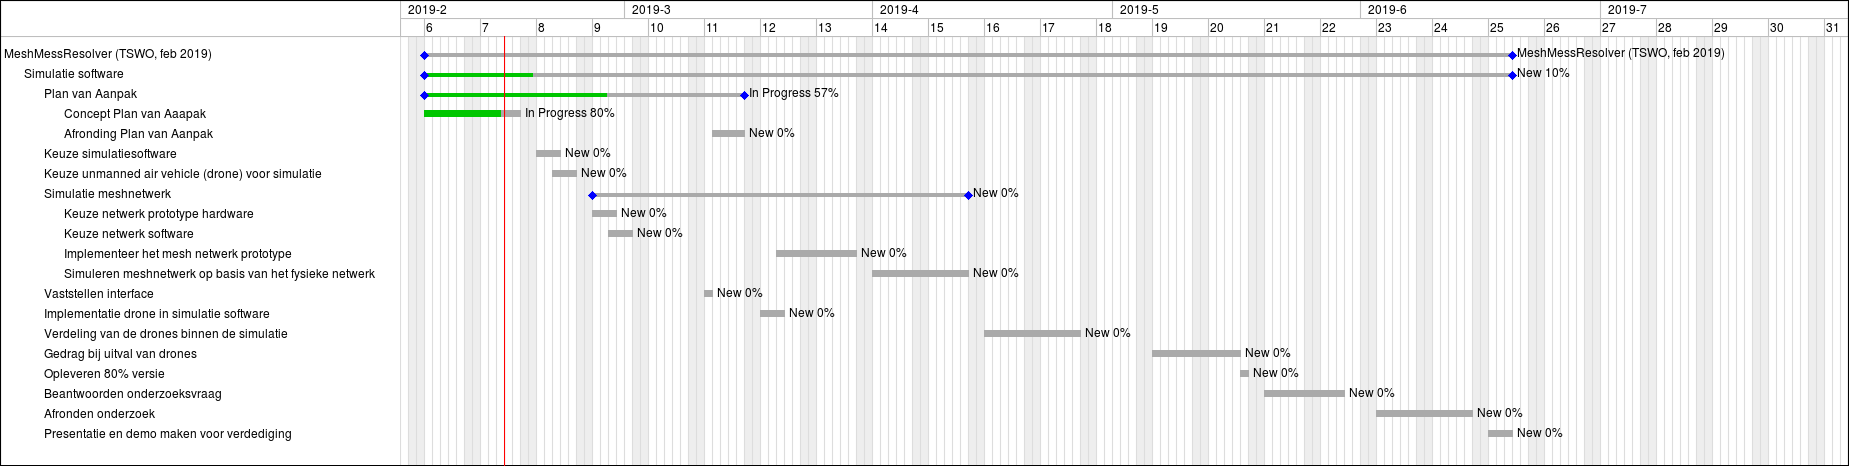
\includegraphics[width=1.1\linewidth]{gantt}\end{center}
	\caption{Gantt chart}
	\label{fig:gantt}
\end{figure}


\chapter{Risico's}
\label{chapter:risicos}
In dit hoofdstuk worden risico's van het project beschreven die niet afgevangen kunnen worden door de student. Er zal een scheiding gemaakt worden tussen risico's die intern kunnen optreden en welke van buitenaf komen. Onderkende risico's die wel afgevangen kunnen worden staan ook genoteerd.

\section{Interne risico's}

\begin{longtable}[c]{|l|l|l|l|l|}
\hline
\rowcolor[HTML]{C0C0C0} 
Risico                                                                                                                                                 & Kans  & Impact & Tegenmaatregel                                                                                                                                                                                                                                                                              & Uitwijkstrategie                                                                                                          \\ \hline
%\endfirsthead
%
\endhead
%
\begin{tabular}[c]{@{}l@{}}Planning voor het \\ onderzoek wordt \\ niet behaald.\end{tabular}                                                          & Groot & Groot  & \begin{tabular}[c]{@{}l@{}}De planning laten\\ reviewen door de\\ begeleiders of naar\\ haalbaarheid. \\ MoSCoW planning\\ gebruiken voor de\\ requirements. Tijdens \\ het project een Gantt\\ chart gebruiken voor\\ om zo vroeg mogelijk\\ achter dit probleem \\te  komen. Sprints \\gebruiken i.c.m. een\\ burndown chart\end{tabular} & \begin{tabular}[c]{@{}l@{}}Requirements die in\\ de could planning \\ vallen schrappen.\end{tabular}                      \\ \hline
	\begin{tabular}[c]{@{}l@{}}Simulatie software \\ is niet toereikend\\ voor het onderzoek.\end{tabular}                                     & Klein  & Groot  & \begin{tabular}[c]{@{}l@{}}Requirements van uit\\ het onderzoek halen\\ waar de\\  simulatiesoftware \\ aan moet voldoen. De \\ \nameref{sec:inceptionfase} moet\\ dit voorkomen.\end{tabular}                                                                                                                     & \begin{tabular}[c]{@{}l@{}}Heronderzoeken welke\\ simulatiesoftware\\ wel toereikend is. \\ Wanneer de beschikbare\\ tijd het toestaat \\ overstappen.\\ Anders moeten de\\ requirements opnieuw \\ overwogen worden.\end{tabular}                                                                           \\ \hline
\caption{Interne risico's}
\end{longtable}

\section{Externe risico's}

\begin{table}[H]
	\centering
	\begin{tabular}{|l|l|l|l|l|}
		\hline
		\rowcolor[HTML]{C0C0C0} 
		Risico                                                                                   & Kans  & Impact & Tegenmaatregel                                                                                                                                    & Uitwijkstrategie                                                                                       \\ \hline
		\begin{tabular}[c]{@{}l@{}}Hardware voor\\ prototype mesh\\ netwerk defect.\end{tabular} & Klein & Groot  & \begin{tabular}[c]{@{}l@{}}Hardware gebruiken\\ die snel leverbaar is.\\ Reserve hardware\\ bestellen als het\\ budget het toestaat.\end{tabular} & \begin{tabular}[c]{@{}l@{}}Andere hardware die\\ aan de requirements\\ voldoet gebruiken.\end{tabular} \\ \hline
	\end{tabular}
\caption{Externe risico's}
\end{table}

\section{Afgevangen risico's}
Onderstaande risico's zijn afgevangen aangezien de student tegenmaatregelen heeft getroffen voor de risico's. Als een van onderstaande risico optreedt weet de student wat er van hem verwacht wordt en wordt de impact van het risico geminimaliseerd.

\begin{longtable}{|l|l|l|l|l|}
	\hline
	\rowcolor[HTML]{C0C0C0} 
	Risico                                                                                                                                     & Kans   & Impact & Tegenmaatregel                                                                                                                                                                                                                                                                                              & Uitwijkstrategie                                                                                                                                                                                                                                                                \\ \hline
	%\endfirsthead
	%
	\endhead
	%
	\begin{tabular}[c]{@{}l@{}}Kwaliteit van\\ producten wordt\\ niet gewaarborgd.\end{tabular}                                                & Klein  & Middel & \begin{tabular}[c]{@{}l@{}}Kwaliteitseisen opstellen\\ in het plan van aanpak.\\ Daarbij wordt ieder\\ product gereviewed door\\ de bedrijfsbegeleider. \\ Het wordt op een later\\ moment nogmaals\\ gereviewed door de\\ student om te kijken\\ of de code voldoet\\ aan de gestelde eisen.\end{tabular} & \begin{tabular}[c]{@{}l@{}}Als er producten zijn \\ die alsnog niet voldoen \\ aan de kwaliteitseisen \\ zal de bedrijfbegeleider\\ actie ondernemen. \\ Hierdoor voldoen alle\\ producten aan de\\ gestelde kwaliteitseisen.\end{tabular}                                      \\ \hline
	\begin{tabular}[c]{@{}l@{}}Langdurige\\ afwezigheid\\ begeleiding.\end{tabular}                                                              & Klein  & Middel  & \begin{tabular}[c]{@{}l@{}}Na een week van geen\\ gehoor stelt de student\\ een ultimatum.\end{tabular}                                                                                                                                                                                                                                                                                                     & \begin{tabular}[c]{@{}l@{}}De organistatie van de\\ begeleider biedt een \\ tijdelijke vervanger aan.\end{tabular}                                                                                                                                                              \\ \hline
	\begin{tabular}[c]{@{}l@{}}Plan van aanpak\\ onderdeel blijkt niet\\  goed geformuleerd\\ of niet (goed)\\ omvattend te zijn.\end{tabular} & Middel & Middel & \begin{tabular}[c]{@{}l@{}}Laten reviewen door\\ begeleiders en docenten\\ of onderdelen correct\\ worden afgevangen.\\ Daarbij ieder hoofdstuk\\ naast het document\\ \APACcitebtitle{Toelichting op PvA 3.0} \\ houden en dit document\\ als een checklist \\ gebruiken.\end{tabular}                                          & \begin{tabular}[c]{@{}l@{}}Plan van Aanpak \\ onderdeel aanpassen\\ zodat het onderdeel\\ correct wordt\\ geformuleerd. Dit\\ onderdeel wordt\\ dan ook nogmaals\\ gereviewd en wordt\\ naast de checklist \\ gehouden, zoals\\ beschreven in de\\ tegenmaatregel.\end{tabular} \\ \hline
\caption{Afgevangen risico's}
\end{longtable}


\bibliographystyle{apacite}
\bibliography{bilbliography.bib}

\clearpage
\appendix
\chapter{Code guideline}
\label{app:code}
In deze bijlage is de code guideline opgesteld, deze is gebasseerd op de google C++ Styleguide (\href{https://google.github.io/styleguide/cppguide.html}{link}) en die van Lockheed Martin (\href{http://www.stroustrup.com/JSF-AV-rules.pdf}{link}) 
\section{Algemeen}

\begin{itemize}
\item Het bestand waar de main functie in zit mag alleen main.cpp genoemd worden en geen andere functies bevatten.
\item Alle source files hebben een header file met uitzondering van main.cpp. Dit zijn .hpp bestanden.
\item Headers alleen includeren in het header/source bestand waar het niet zonder kan.
\item Zowel commentaar als code zijn in het Engels geschreven.
\item Volgorde van includeren: system, library, local. Wordt gescheiden met een witregel.
\item Het gebruik van verouderde .h libraries is verboden. Gebruik hiervoor de c++ variant. Bijvoorbeeld $<$cmath$>$ ipv $<$math.h$>$
\item Bij if, else, while, do en for instructies altijd accolades gebruiken. Accolade openen op de volgende regel.
\item Geen onnodig witregels. Binnen een codeblok is er maximaal één opeenvolgend witregel toegestaan. Daarbuiten zijn er maximaal twee toegestaan.
\item Code die niet wordt gebruikt of is uitgecommentarieerd wordt verwijderd.
\item Maximale aantal tekens per rij is 80 regels. Uitzonderingen hierop als er gebruik wordt gemaakt van raw String data, deze zullen niet meetellen in het aantal karakters.
\item Foutmeldingen alleen in de vorm van exeptions/runtime errors. Het gebruik van return fouten (illegale Int \& bool) is verboden.
\end{itemize}

\section{Class, Struct en Enum}
\begin{itemize}
\item Accolades op een nieuwe regel.
\item Een class representeert niet meer dan één samenstelling van bij elkaar horende eigenschappen.
\item De constructor van een class mag naast het zetten van variabelen geen uitgebreid rekenwerk uitvoeren. Dit wordt gedaan in een aparte functie bijvoorbeeld void init.
\item Struct mag voor passieve objecten die alleen data dragen, anders wordt het een class.
\item Maak alle waarden en functies Private wanneer dit kan.
\end{itemize}

\section{Functies}
\begin{itemize}
\item Commentaar over wat een functie doet staat in de header. Uitleg over de werking ervan staat in de source file.
\item Een functie heeft niet meer dan één doel. Aan de hand van het commentaar is dit doel duidelijk.
\item Accolades op een nieuwe regel.
\item De scope van een functie is zo klein mogelijk.
\item Parameters die niet gewijzigd worden binnen de functie zijn als const aangeduid alleen wanneer er geen sprake is van "pass by value".
\item Probeer forward declerations zoveel mogelijk te vermijden.
\item Inline functies mogen niet groter zijn dan 1 regel.
\item Voor elke functie, die wat berekend of wat retourneerd, worden unittests voor geschreven. Getters en setters hoeven niet.
\item Mocht de functie moeten werken in een thread, heeft deze zijn eigen try en catch.
\end{itemize}

\section{Variabelen}
\begin{itemize}
\item Bij een pointer declaratie wordt de asterisk tegenaan de datatype gezet.
\item Bij een reference declaratie wordt de ampersand tegenaan de datatype gezet.
\item De scoop van een variabele is zo klein mogelijk.
\item Alle variabelen worden geinitialiseerd voor gebruik.
\end{itemize}
\section{Naamgeving}
\begin{itemize}
\item Naamgeving in lowerCamelCase, tenzij expliciet anders vermeld.
\item Constante waarden (\#define, const declaratie en enum members) in hoofdletters met een laag liggend streepje tussen de woorden.
\item Class, struct, enum, union en typedef namen UpperCamelCase.

\end{itemize}
\section{Commentaar}

\begin{itemize}
\item Commentaar wordt geschreven in Doxygen format.
\item In de tag @brief wordt beschreven welk doel de class behaald.
\item In de tag @author wordt gezet wie de functie heeft gemaakt.
\item In de tag @param worden de parameters beschreven van de functie. 
\item In de tag @return wordt beschreven wat de functie retourneert.
\item Commentaar voor een functie hoeft niet in een @brief tag worden beschreven.
\item In de beschrijving van de functie een pre en post conditie van de functie benoemen. Bij get en set is dit niet verplicht. 
\item Commentaar moet enkel gaan over code en niet over ontwerpen of andere externe bronnen.
\item Commentaar wordt geschreven boven de functie. Deze is alleen nodig wanneer het toegevoegde waarde heeft.
\item Commentaar wordt geschreven boven of naast de variabele. Deze is alleen nodig wanneer het toegevoegde waarde heeft.
\end{itemize}

\chapter{Iteratie plan template}
\label{app:iteratieplan}

\begin{center}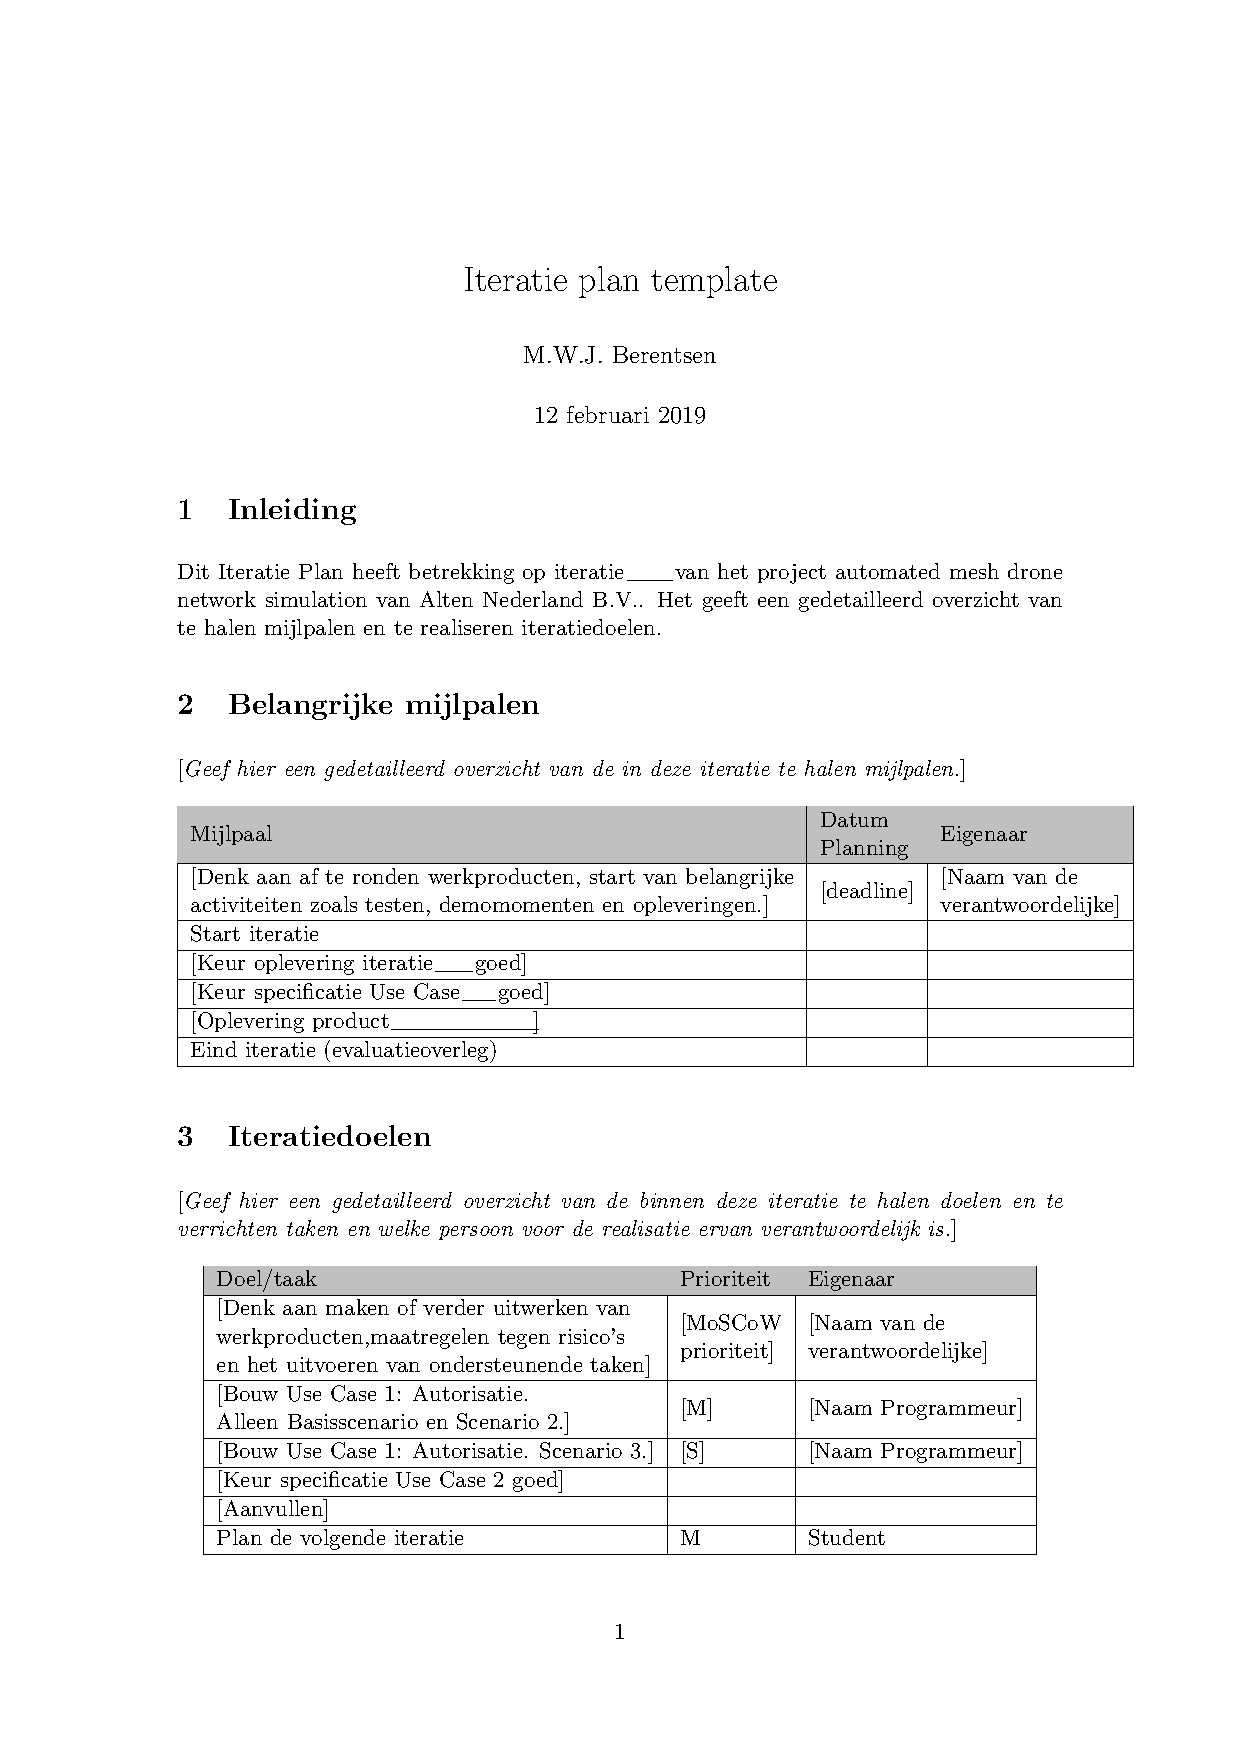
\includegraphics[page=1,width=.8\linewidth]{Templates/Iteratieplan/Iteratieplan.pdf}\end{center}
.$\backslash$Templates$\backslash$Iteratieplan.pdf

\chapter{Iteratie assessment template}
\label{app:assesement}

\begin{center}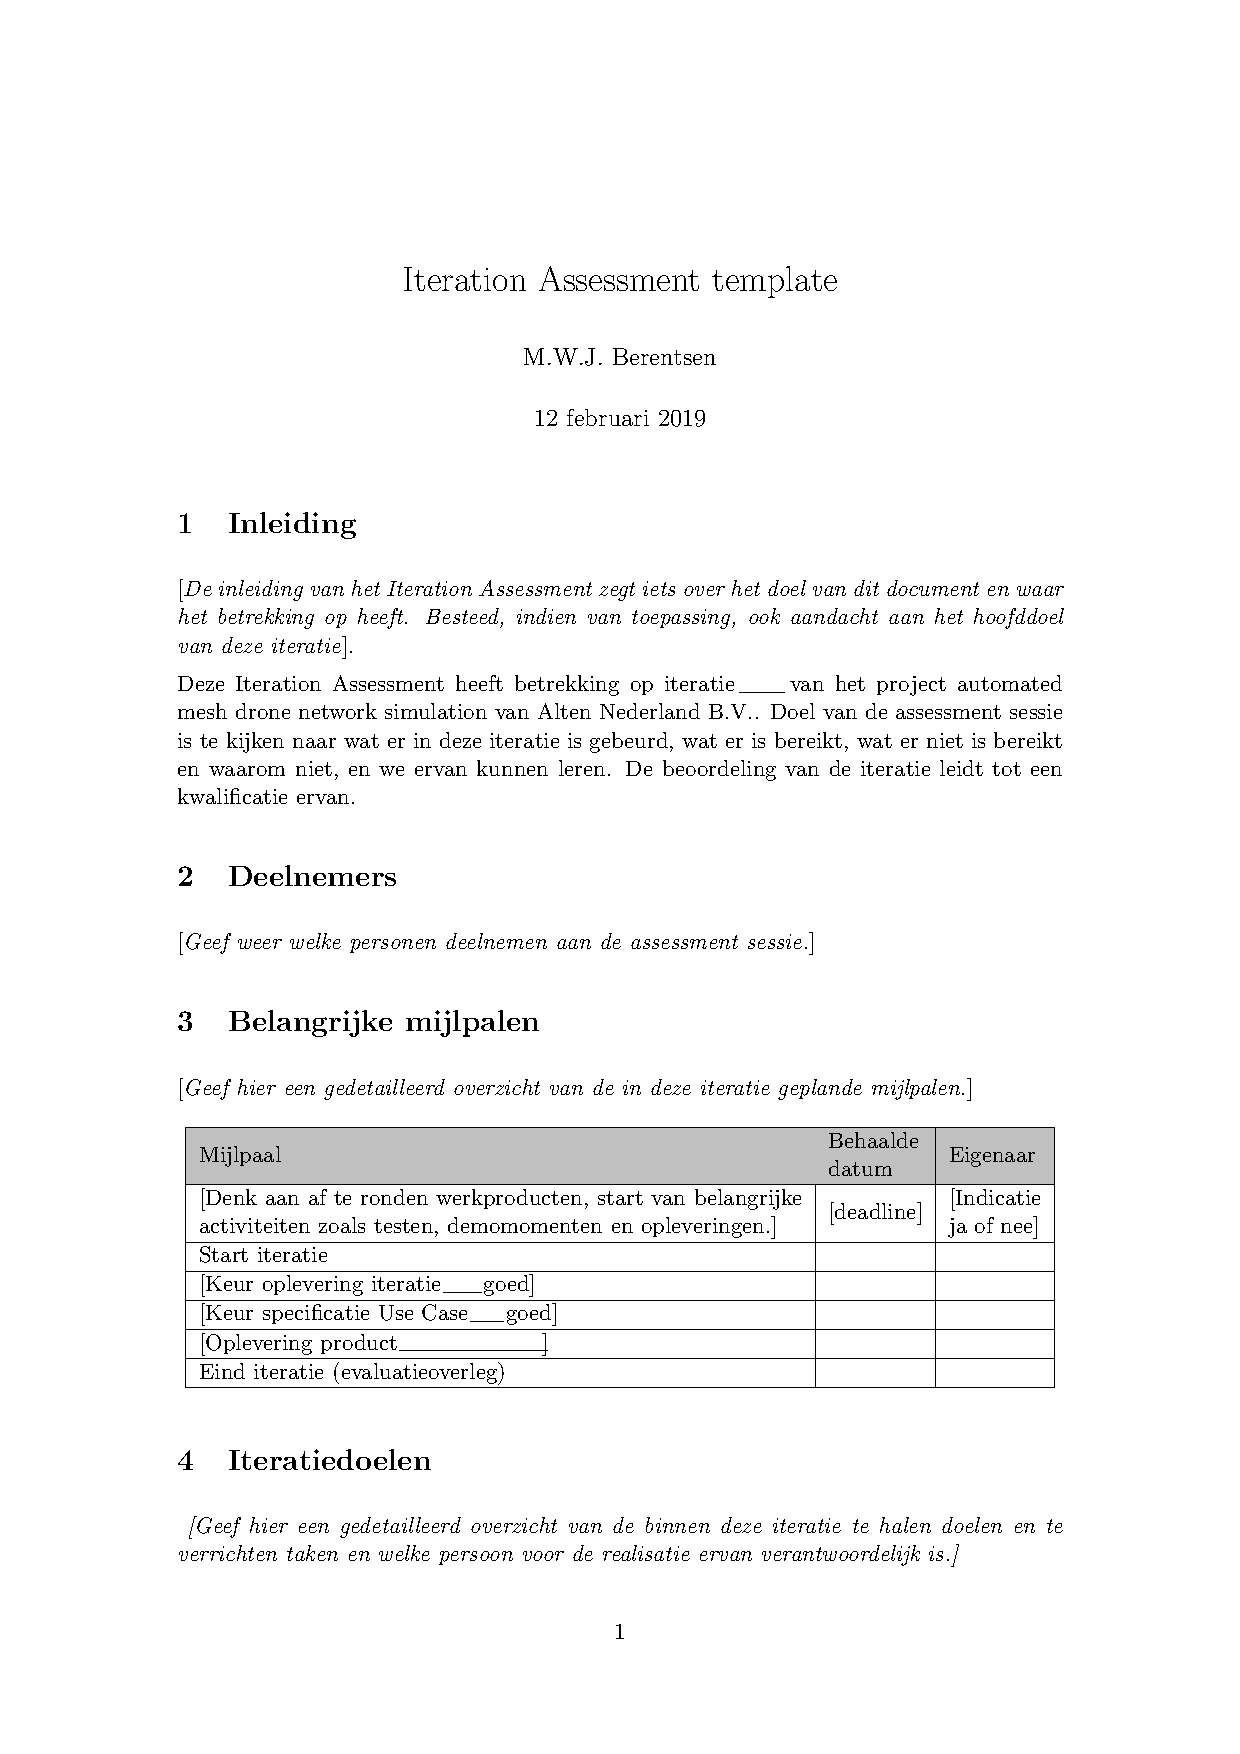
\includegraphics[page=1,width=.8\linewidth]{Templates/Ieteratieassessement/IterationAssessment.pdf}\end{center}
\begin{center}\includegraphics[page=2,width=.8\linewidth]{Templates/Ieteratieassessement/IterationAssessment.pdf}\end{center}
.$\backslash$Templates$\backslash$IterationAssessment.pdf


\chapter{Usecase template}
\label{app:usecasetemplate}

\begin{center}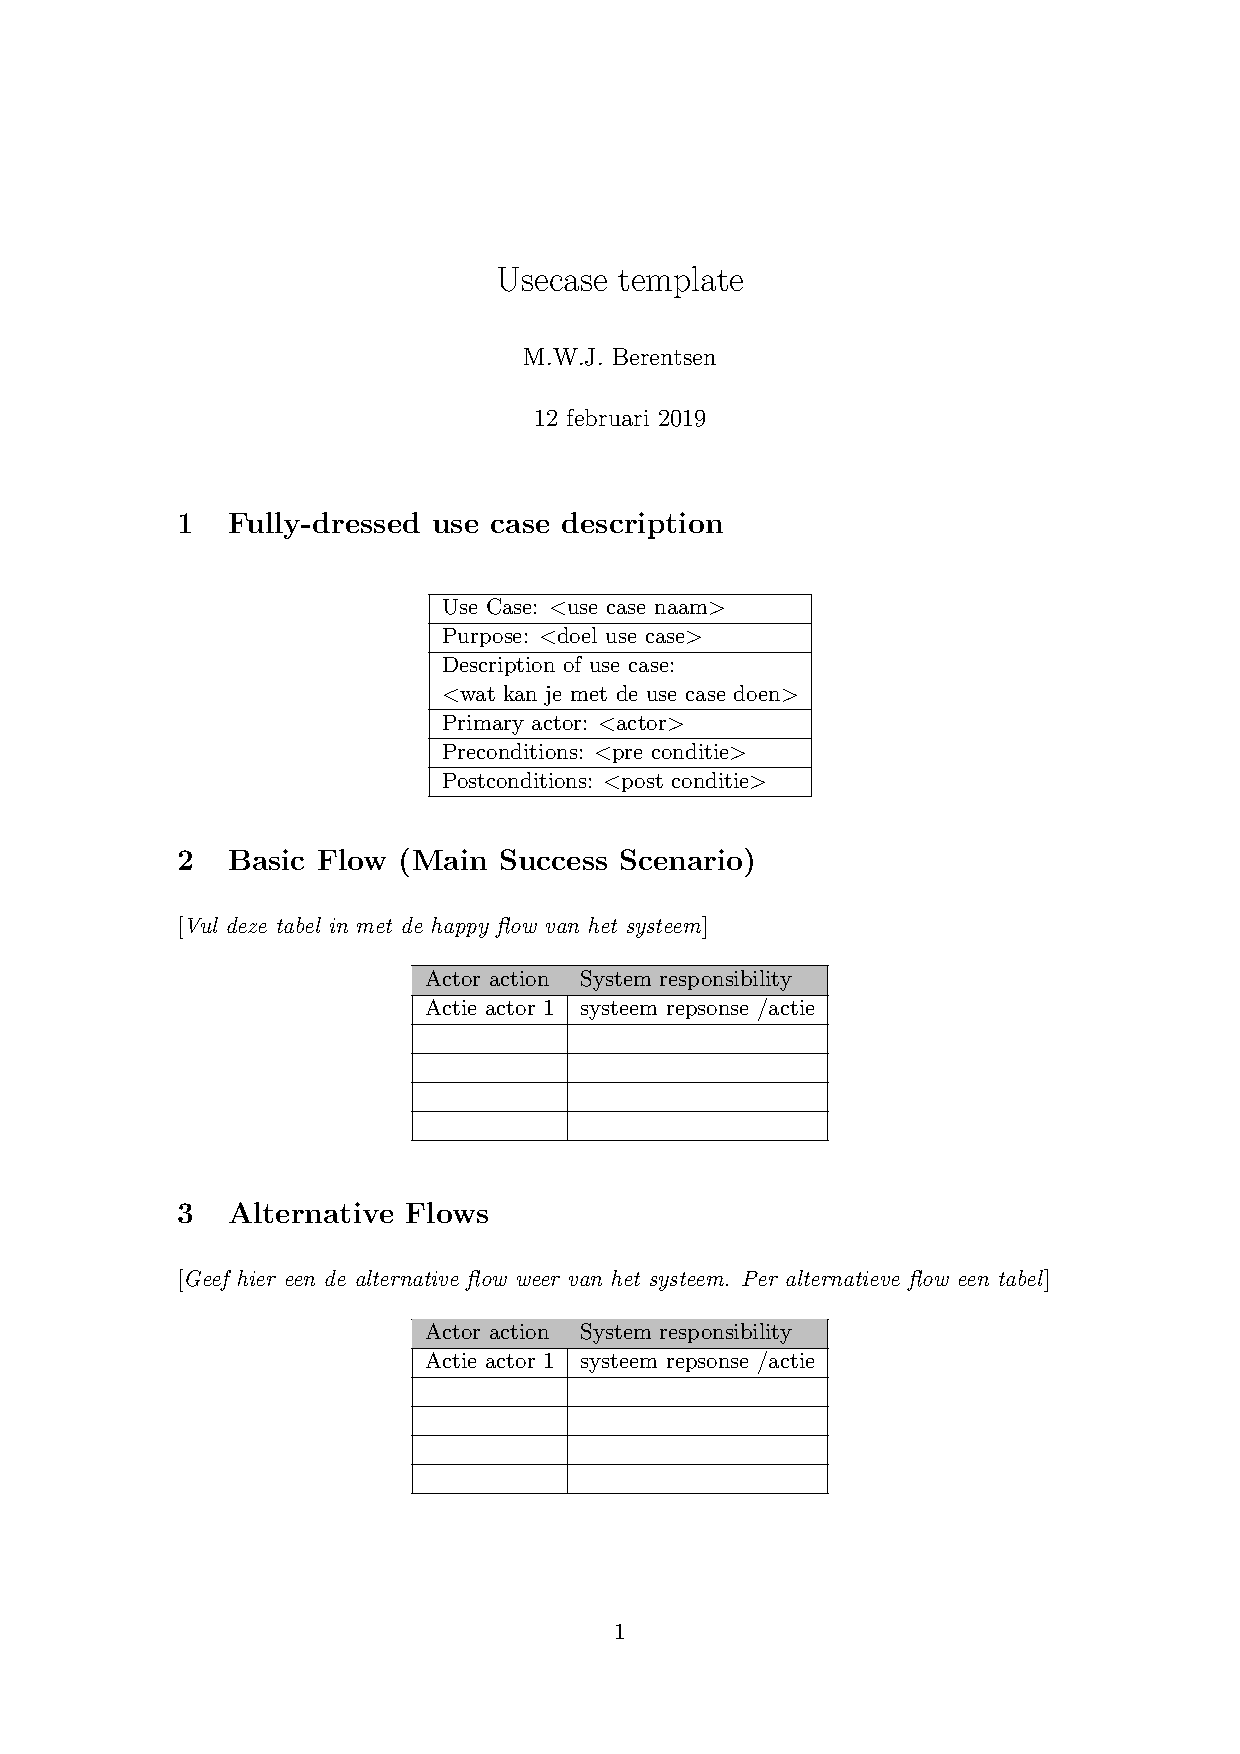
\includegraphics[page=1,width=.8\linewidth]{Templates/Usecase/usecasetemplate.pdf}\end{center}
.$\backslash$Templates$\backslash$usecasetemplate.pdf

\chapter{Definition of Done}
\label{app:DoD}
Voor elke programmeer taak is een gelijke definition of done opgesteld.
Dit is een simpele checklist om de programmeur scherp te houden of het opgeleverde werk ook echt af is.
Deze lijst zal in de taken op redmine terug te vinden zijn.

\begin{itemize}
	\item Documentatie voldoet aan gestelde eisen.
	\item Ontwerpen voldoen aan gestelde eisen.
	\item Code getest.
	\item Code voldoet aan Code style guideline.
	\item Code gedocumenteerd (Doxygen).
	\item Code compileert.
	\item Code doet wat het moet doen.
\end{itemize}




\end{document}